\chapter{Preliminares}\label{chapter:REV-LL}

Este trabajo pretende implementar un sistema que resuelva instancias de VRP en cualquiera de sus variantes con el menor trabajo humano posible. En este capítulo se presentan los principales elementos de la investigación realizada para lograrlo.

Primeramente se comienza con una visión general del problema de enrutamiento de vehículos (VRP) y algunas de sus variantes con la sección \ref{2-VRPintro}. Se explica cómo describir a partir de código una solución de VRP.

 En \ref{2-Libr} se muestran las bibliotecas de clases existentes hasta el momento que pueden ser utilizadas para encontrar soluciones a instancias de VRP.
 
En \ref{2-Hector} se explica cómo crear un Árbol de vecindad a partir de una solución inicial y un criterio de vecindad. Este árbol es utilizado para obtener la cardinalidad de vecindades y realizar una exploración de dos fases que utiliza técnincas estadísticas.

En \ref{2-JJ} se expone el concepto de Grafo de evaluación y cómo es esto utilizado para evaluar soluciones de forma eficiente y automática.

En \ref{2-Heidy} se presenta un mecanismo para explorar vecindades de forma automática a partir de combinaciones de cualesquiera estrategias de exploración y selección.

Finalmente en \ref{2-Lisp} se describe brevemente algunas características y funcionalidades del lenguaje Common Lisp que resultaron especialmente útiles para el desarrollo del sistema.


%\newpage

\section{Problema de Enrutamiento de Vehículos}\label{2-VRPintro}
La primera referencia al VRP fue hecha por Dantzing y Ramser en \cite{Ramsin1959} en el año 1959. Se propone una formulación matemática, una aproximación algorítmica y se describe una aplicación real entregando gasolina a varias estaciones de servicio. 

En su versión más simple, el problema consta de una flota de vehículos que salen de un depósito y deben satisfacer las demandas de una serie de clientes. El objetivo es encontrar una distribución de caminos a asignar a los vehículos de forma que se optimice determinada métrica (tiempo, combustible, etc). Con más de 50 años de estudios se ha ramificado en una inmensa cantidad de variantes entre las que se pueden contar las siguientes:

\begin{itemize}
	\item CVRP - VRP con restricciones de capacidad. Cada vehículo tiene una capacidad que no debe ser excedida.
	\item VRPTW - VRP con ventanas de tiempo. Cada cliente posee un período de tiempo fijo durante el cual puede ser atendido.
	\item VRPPD - VRP con recogida y entrega. Los bienes deben ser entregados y recogidos en cantidades fijas.
	\item MDVRP - VRP con múltiples depósitos. Se cuenta con múltiples depósitos desde los que pueden salir los vehículos.
\end{itemize}

Esta es una familia de problemas NP-Duros, por lo las soluciones exactas no son factibles para instancias de grandes tamaños. Para buscar aproximaciones a la solución se utilizan heurísticas y metaheurísticas. Se destaca la búsqueda local como metaheurística que ha dado muy buenos resultados y es la seleccionada en el presente trabajo como se explica en \ref{2-Local}.

\subsection{Representación de soluciones del VRP}\label{2-Sol}
Las soluciones son representadas (en su versión más simple) como una serie de listas de clientes denominadas rutas.
Si se define a $P_1$ como un problema clásico que consta de 6 clientes: $[c_1, c_2, c_3, c_4, c_5, c_6]$, entonces una solución $s_1$ se puede definir como:

\begin{equation}
s_1 = [(c_2,c_3), (c_1,c_4,c_5), (c_6)]
\end{equation}

En $s_1$ se representa una solución con tres rutas. El vehículo perteneciente a la primera ($r_1$) ruta visita a $c_2$ y $c_3$, el vehículo de la segunda ruta ($r_2$) visita a $c_1$, $c_4$ y $c_5$ y el de la tercera ($r_3$) sólo visita a $c_6$.


\subsection{Metaheurísticas de búsqueda local}\label{2-Local}
Los algoritmos basados en búsquda local son aquellos en que se define una solución inicial y a partir de determinado criterio de vecindad se busca la solución óptima iterando por los vecinos de la vecindad formada por dicho criterio. A continuación se muestran algunos ejemplos de criterios de vecindad:

\begin{enumerate}
	\item Cambiar de posición a un cliente dentro de su ruta.
	\item Mover a un cliente de ruta.
	\item Intercambiar dos clientes de posición.
	\item Cambiar vehículo de ruta.
	\item intercambiar dos subrutas entre sí.
	\item invertir orden de una subruta. 
\end{enumerate}

Los criterios de vecindad dependen también de la variante del problema sobre la que se trabaje. Por ejemplo, el criterio de \textbf{"Cambiar vehículo"} no tiene sentido para el problema $P_1$ pues en este todos los vehículos son iguales.

Estas operaciones pueden ser obtenidas a partir de un subconjunto de operaciones más simples a las que se denomina operaciones elementales. Entre las operaciones elementales se encuentran: \textbf{selección de ruta}, \textbf{selección de cliente} e \textbf{inserción de cliente}.

Por ejemplo, \textbf{intercambiar dos clientes de posición} puede ser realizado a partir de dos \textbf{selección de ruta}, dos \textbf{selección de cliente} y dos \textbf{inserción de cliente}.

La importancia de las operaciones elementales para la implementación del sistema se explicarán en con más profundidad en \ref{label}.

A partir de un criterio y una solución inicial se pueden generar nuevas soluciones. El proceso de obtención y selección de nuevas soluciones se denomina exploración de la vecindad. Mientras más grande la vecindad es más probable encontrar mejores soluciones, pero esto puede requerir una gran cantidad de tiempo. Por tanto, las estrategias a seguir durante la exploración son un factor vital a tener en cuenta para la implementación del sistema y se explicarán en \ref{2-Hector} y \ref{2-Heidy}. Además, a la hora de comparar el costo entre dos soluciones es necesario evaluarlas, lo cual posee también un costo computacional considerable. Para la evaluación de soluciones se tiene el Grafo de evaluación explicado en \ref{2-JJ}.

\section{Vías de solución existentes}\label{2-Libr}
Una buena herramienta para resolver problemas de VRP en la actualidad es la biblioteca OR-Tools (Google Optimization Tools). Un software de código abierto útil para problemas de optimización combinatoria entre los que se encuentra el Problema de Enrutamiento.

NOTA PARA FERNANDO: Profe, no sé qué más poner aquí XD.

\section{Combinación de estrategias de exploración y selección.}\label{2-Heidy} 
TODO

\section{Árbol de vecindad y exploración de dos fases}\label{2-Hector}
La exploración de vecindades puede ser ineficiente y difícil de programar. La idea que se propone es utilizar técnicas estadísticas para analizar cuáles son las mejores regiones de las vecindades para intensificar la búsqueda en estas.

Buscando aplicar dichas técnicas estadísticas es necesario saber la cardinalidad de las vecindades y separarlas en regiones. Para lograr esto de forma eficiente (sin iterar por todos los elementos de una vecindad) se propone la creación de un Árbol de vecindad. El Árbol de vecindad utiliza oun concepro de $solucion$ diferente al explicado en \ref{2-Sol}. Previamente se definió una solución de VRP en su forma más trivial como una lista de caminos conformados a su vez por la lista de clientes que se visitan en cada uno, por ejemplo:

\begin{equation}
s_1 = [(c_2,c_3), (c_1,c_4,c_5), (c_6)]
\end{equation}

Con el propósito de contar la cantidad de soluciones que tiene una vecindad, pierde importancia saber qué clientes se visita en cada ruta, en cambio sólo es necesario conocer la cantidad de clientes visitados en cada una. A este tipo de solución se le denomina solución de conteo y aplicado a $s_1$ daría como resultado:

\begin{equation}
sc_1 = [2, 3, 1]
\end{equation}

Teniendo una solución inicial, todas las soluciones de una vecindad pueden ser obtenidas aplicando sobre esta el criterio de vecindad en cuestión, con todos sus valores posibles. A la asignación de valores de un criterio de vecindad sobre una solución se le llamará una instanciación de dicho criterio. Por ejemplo, dado el criterio \textbf{mover cliente} dado por: 

\begin{itemize}
	\item Seleccionar ruta (r).
	\item Seleccionar cliente en ruta (a).
	\item Seleccionar ruta (r).
	\item Insertar cliente en ruta (b).
\end{itemize}
Las letras $r$, $a$ y $b$ son los símbolos representativos de cada operación.

Un ejemplo de instanciación de este criterio sobre la solución $s_1$ se presenta como:

\begin{itemize}
	\item $r_1 = 1$ $\rightarrow$ $r_1$ es la ruta de la que el cliente $c_1$ es extraído.
	\item $c_1$.position = 1 $\rightarrow$ $c_1$ es el primer cliente de la ruta.
	\item $r_2 = 1$ $\rightarrow$ $r_2$ es la ruta de la que el cliente $c_1$ será insertado.
	\item $c_1$.position = 2 $\rightarrow$ $c_1$ es insertado en la posición 2 de la ruta seleccionada.
\end{itemize}

A cada vecino de un criterio se le puede hacer corresponder una instanciación del mismo y por tanto, encontrar la cardinalidad de una vecindad es similar a encontrar el número de instanciaciones posibles del criterio asociado.

Al generar las distintas instanciaciones de un criterio de vecindad para
una solución dada se cumple que muchas de estas comparten una secuencia común de operaciones instanciadas. La estrategia propuesta se basa en
agrupar aquellos criterios instanciados para los cuales dicha secuencia común comience en la primera operación de los mismos, pues de esta forma
el resto de las operaciones de tales criterios instanciados no se ven afectadas, y contar para cada una de estas el número de posibles secuencias de operaciones instanciadas que unidas con la secuencia común forman un
criterio instanciado.

Al computar la cardinalidad de una vecindad del VRP, se utiliza una
estrategia recursiva que consiste en contar para una operación el número
de secuencias de operaciones instanciadas que se pueden formar con el
resto de las operaciones del criterio, así como combinar las mismas con
las posibles instanciaciones de la operación actual aprovechando que para
las operaciones modificadoras estas secuencias son comunes a todas las
posibles instanciaciones de las mismas.

Es posible utilizar este algoritmo, para almacenar toda la información
necesaria para cualquier procesamiento posterior sobre dicha vecindad en
una estructura arbórea que será llamada árbol de vecindad y que constituye
una representación de la vecindad en cuestión. En \ref{fig:neigh-tree} se muestra una representación del árbol de vecindad asociado a l criterio \textbf{mover cliente} ($rarb$). Cada nodo del árbol, representa una
operación de vecindad y almacena toda la información necesaria para instanciar dicha operación y de esta forma, a partir del proceso que computa
la cardinalidad de la vecindad, se pueden pasar a generar todas las soluciones de la misma.


% TODO: \usepackage{graphicx} required
\begin{figure}
	\centering
	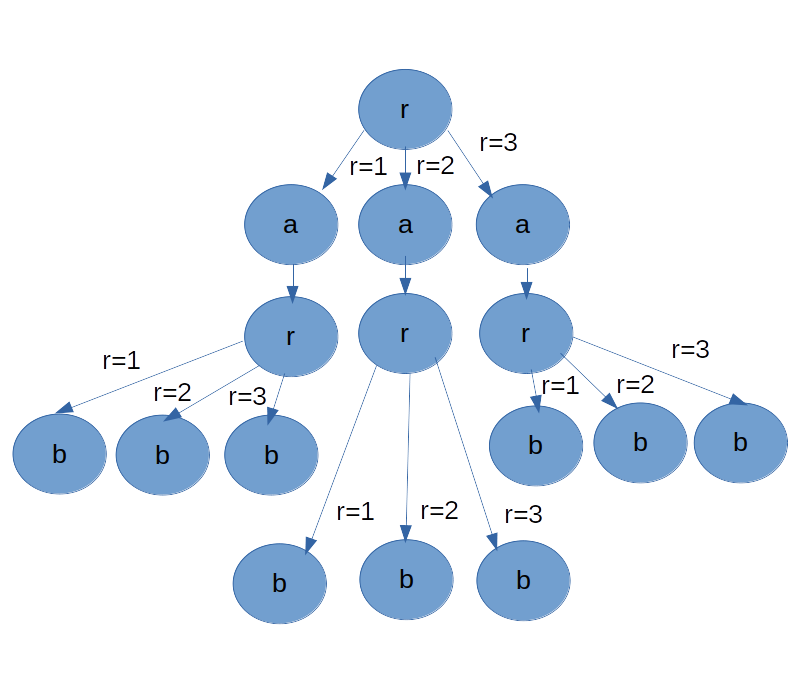
\includegraphics[width=0.9\linewidth]{Graphics/Neigh-Tree}
	\caption{Árbol de vecindad asociado a $rarb$}
	\label{fig:neigh-tree}
\end{figure}

Cada rama del árbol representa un conjunto de soluciones, por tanto, el conjunto de ramas representa una partición de la vecindad a la que está asociado dicho árbol. A los conjuntos hechos por esta partición se les denomina regiones y resultan útiles para encontrar características compartidas en grupos de vecindades. Por ejemplo, es conveniente analizar cuáles son las regiones con mejores soluciones para intensificar en estas la búsqueda de soluciones óptimas.

La exploración en dos fases es una heurística útil para explorar una vecindad de un VRP realizando el análisis de la misma en dos etapas. Una primera, llamada de exploración, donde se intenta construir una muestra representativa de la vecindad en cuestión, y otra etapa posterior de explotación (o de intensificación), en la cual se exploran las regiones más prometedoras de la vecindad que fueron identificadas mediante el uso de ténicas estadísticas sobre la muestra generada en la fase anterior.


\section{Grafo de Evaluación}\label{2-JJ}
TODO

\section{Common Lisp y sus funcionalidades}\label{2-Lisp}
Common Lisp es un lenguaje de programación multi paradigma (soporta una combinación de paradigmas de programación tales como la programación imperativa, funcional y orientada a objetos). Facilita el desarrollo de software evolutivo e incremental, con la compilación iterativa de programas eficientes en tiempo de ejecución.

NOTA PARA FERNANDO: Tampoco sé muy bien qué decir aquí. Pensaba en explicar el modo .org y cómo se van tangleando los scripts y eso, pero me parece que eso es emacs, ¿no? *emoji pensativo*. O puedo hablar de lo útil que resulta la herencia múltiple para definir las clases a partir de la combinación de varias clases abstractas y cómo se usa esto después en los métodos para ver qué especializaciones usar... Pero en esta parte me parece violación pues no he explicado nada de código *otro emoji pensativo*



























